% 手拉手等边特例：两个共顶点等边三角形 △OAB（上方）、△OCD（右方）
% 红虚线 AC、BD 应等长且夹角 60°
\documentclass[tikz,border=4pt]{standalone}
\usepackage{ctex}
\usepackage{amsmath}
\usetikzlibrary{calc, decorations.markings}
\begin{document}
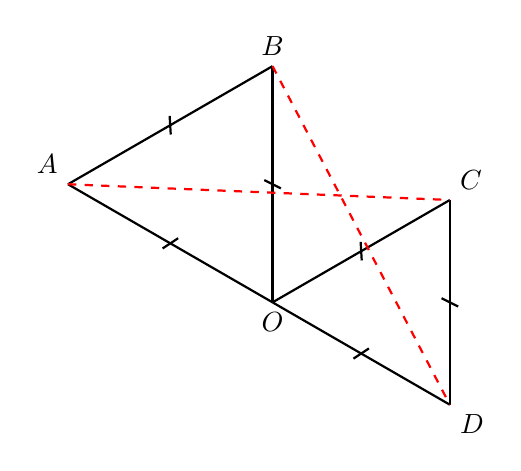
\begin{tikzpicture}[scale=1.0, thick,
  tick/.style={postaction={decorate, decoration={markings,
    mark=at position 0.5 with {\draw (-1.5pt,-3pt) -- (1.5pt,3pt);}}}}]

  \coordinate (O) at (0, 0);
  % △OAB 在上方：OA 朝 150°、OB 朝 90°（夹角 60°），边长 3
  \coordinate (A) at ({3*cos(150)}, {3*sin(150)});
  \coordinate (B) at ({3*cos(90)},  {3*sin(90)});
  % △OCD 在右方：OC 朝 30°、OD 朝 -30°（夹角 60°），边长 2.6
  \coordinate (C) at ({2.6*cos(30)},  {2.6*sin(30)});
  \coordinate (D) at ({2.6*cos(-30)}, {2.6*sin(-30)});

  \draw[tick] (O) -- (A);
  \draw[tick] (O) -- (B);
  \draw[tick] (A) -- (B);
  \draw[tick] (O) -- (C);
  \draw[tick] (O) -- (D);
  \draw[tick] (C) -- (D);

  \draw[red, dashed] (A) -- (C);
  \draw[red, dashed] (B) -- (D);

  \node[below]       at (O) {$O$};
  \node[above left]  at (A) {$A$};
  \node[above]       at (B) {$B$};
  \node[above right] at (C) {$C$};
  \node[below right] at (D) {$D$};
\end{tikzpicture}
\end{document}
